\section{Homework 3: Categorical Data Analysis}

\subsection{Problem 1}

Suppose that all cell counts $\{n_{ij}\}$, $i = 1, \ldots, I$ and $j = 1, \ldots, J$, follow a multinomial distribution with a fixed total count $n$ and proportion parameters $\{\pi_{ij}\}$. Write the likelihood function and solve for the MLE.

\textbf{解答：}

Likelihood:
\[
L(\{\pi_{ij}\}) = \frac{n!}{\prod_{i=1}^{I} \prod_{j=1}^{J} n_{ij}!} \prod_{i=1}^{I} \prod_{j=1}^{J} \pi_{ij}^{n_{ij}}
\]

取对数：
\[
\log L(\{\pi_{ij}\}) = \text{const} + \sum_{i,j} n_{ij} \log \pi_{ij}
\]

已知约束 $\sum_{i,j} \pi_{ij} = 1$，由 Lagrange 乘因子法，令
\[
F = \sum_{i,j} n_{ij} \log \pi_{ij} - \lambda \left(1 - \sum_{i,j} \pi_{ij}\right)
\]

对 $\pi_{ij}$ 求偏导并令其为 0：
\[
\frac{\partial F}{\partial \pi_{ij}} = \frac{n_{ij}}{\pi_{ij}} + \lambda = 0 \implies \pi_{ij} = \frac{n_{ij}}{-\lambda}
\]

对所有 $\pi_{ij}$ 求和：
\[
\sum_{i,j} \pi_{ij} = \frac{\sum_{i,j} n_{ij}}{-\lambda} = \frac{n}{-\lambda} = 1 \implies \lambda = -n
\]

因此：
\[
\boxed{\hat{\pi}_{ij}^{\text{MLE}} = \frac{n_{ij}}{n}, \quad \forall\, i, j}
\]

\subsection{Problem 2}

Verify that the ASE for $\log(\widehat{OR}) = [\log(n_{11}) - \log(n_{12})] - [\log(n_{21}) - \log(n_{22})]$ is
\[
\left(\frac{1}{n_{11}} + \frac{1}{n_{12}} + \frac{1}{n_{21}} + \frac{1}{n_{22}}\right)^{1/2}.
\]

Hint: Note that $n_{11} + n_{12} = n_{1.}$ is a fixed row sum. Consider the function of $n_{11}$:
\[
f(n_{11}) = \log(n_{11}) - \log(n_{1.} - n_{11})
\]

\textbf{解答：}

行和为定值，即 Independent multinomial，$n_{11} \sim B(n_{1.}, p)$。

记 $f(n_{11}) = \log n_{11} - \log(n_{1.} - n_{11})$，则
\[
f'(n_{11}) = \frac{1}{n_{11}} + \frac{1}{n_{1.} - n_{11}} = \frac{1}{n_{11}} + \frac{1}{n_{12}}
\]

由 $n_{11} \sim B(n_{1.}, p)$，$\text{Var}(n_{11}) = n_{1.} p(1-p)$。

由 Delta method：
\[
\text{Var}(f(n_{11})) \approx \left(\frac{1}{n_{11}} + \frac{1}{n_{12}}\right)^2 \cdot n_{1.} p(1-p) \xrightarrow{p} \frac{1}{n_{11}} + \frac{1}{n_{12}}
\]

（当 $n \to \infty$ 时，$\frac{n_{11}}{n_{1.}} \to p$）

同理可得
\[
\text{Var}\left[\log\frac{n_{21}}{n_{22}}\right] \xrightarrow{p} \frac{1}{n_{21}} + \frac{1}{n_{22}}
\]

由于行之间独立，故
\[
\boxed{\text{ASE}\left[\log(\widehat{OR})\right] = \left(\frac{1}{n_{11}} + \frac{1}{n_{12}} + \frac{1}{n_{21}} + \frac{1}{n_{22}}\right)^{1/2}}
\]

\subsection{Problem 3}

Consider three smoking behaviors: nonsmoking, smoking $0 < s < 20$ cigarettes per day, and smoking $s \geq 20$ cigarettes per day. An estimated odds ratio for adult females between the presence of squamous cell carcinoma (yes, no) and smoking behavior (smoking $0 < s < 20$ cigarettes per day, nonsmoking) equals 11.7. The estimated odds ratio for adult females between carcinoma (yes, no) and smoking behavior (smoking $s \geq 20$ cigarettes per day, nonsmoking) is 26.1. Show that the estimated odds ratio between carcinoma (yes, no) and the smoking levels ($s \geq 20$, $0 < s < 20$) equals 2.2. Explain how many odds ratios are needed to characterize such a table.

\textbf{解答：}

\[
OR = \frac{n_{11} n_{22}}{n_{12} n_{21}}
\]

因此
\[
OR_{s \geq 20 \text{ vs } 0 < s < 20} = \frac{OR_{s \geq 20 \text{ vs nonsmoking}}}{OR_{0 < s < 20 \text{ vs nonsmoking}}} = \frac{26.1}{11.7} \approx 2.2
\]

独立的 OR 有 $(2-1) \times (3-1) = \boxed{2}$ 个。由上也可见知道其中 2 个可以算出第 3 个。

（对于 $I \times J$ 列联表，独立 OR 有 $(I-1)(J-1)$ 个。）

\subsection{Problem 4}

A researcher attempts to determine if a disease is associated with the presence of a particular gene. He recruited 250 subjects with the disease and 250 normal subjects. The study results showed that 48 subjects have the gene, among whom 30 were diseased subjects.

\subsubsection*{(a)}

Perform a statistical test to investigate whether the disease is associated with the presence of gene.

\textbf{解答：}

\begin{center}
\begin{tabular}{c|cc|c}
 & gene: yes & gene: no & total \\
\hline
disease: yes & 30 & 220 & 250 \\
disease: no & 18 & 232 & 250 \\
\hline
total & 48 & 452 & 500 \\
\end{tabular}
\end{center}

使用 Pearson $\chi^2$ test：$H_0: \pi_{ij} = \pi_{i.} \cdot \pi_{.j}$, $\forall\, i\ \&\ j$, $\alpha = 0.05$

Expected counts：
\[
\hat{\mu}_{11} = \frac{48 \times 250}{500} = 24 = \hat{\mu}_{21}
\]
\[
\hat{\mu}_{12} = \frac{452 \times 250}{500} = 226 = \hat{\mu}_{22}
\]

Statistic：
\[
\chi^2 = \frac{(30 - 24)^2}{24} + \frac{(220 - 226)^2}{226} + \frac{(18 - 24)^2}{24} + \frac{(232 - 226)^2}{226} = 3.32
\]

$\chi^2 \sim \chi^2(1)$，对应临界值 $\chi^2_{0.05}(1) = 3.84 > 3.32$

因此 \textbf{不拒绝 $H_0$}，没有足够理由说明疾病与该基因相关。

\subsubsection*{(b)}

Suppose that we know the following additional information: each of the 250 normal subjects was matched to each of the 250 diseased subjects by gender, race and age group; for 214 matched pairs, neither the diseased subject nor their matched normal subject has the gene. Perform an appropriate statistical test to investigate whether the disease is associated with the presence of the gene.

\textbf{解答：}

\begin{center}
\begin{tabular}{c|cc|c}
 & normal: no & normal: yes & total \\
\hline
disease: no & 214 & 6 & 220 \\
disease: yes & 18 & 12 & 30 \\
\hline
total & 232 & 18 & 250 \\
\end{tabular}
\end{center}

$H_0$ 同 (a)。根据配对数据可以构建如下列联表，使用 McNemar test：
\[
\chi^2 = \frac{(18 - 6)^2}{18 + 6} = \frac{144}{24} = 6 > 3.84
\]
\[
\Rightarrow \text{拒绝 } H_0
\]

认为疾病和基因可能相关。

\subsubsection*{(c)}

Compare the test results in (a) and (b) and explain why they are different.

\textbf{解答：}

解释：未配对时可能忽略了 gender, race, age 等可能的协变量对结果的影响，而配对则考虑了这些信息，增强了 power。

\subsection{Problem 5}

(Framingham study) Consider the binary cholesterol status as the outcome. Test its independence with BMI, age group, and sex, separately, at baseline. For each test, follow the steps below.

(a) Visualize the data using figures or tables.

(b) Specify your selected method and report your $p$-value.

(c) Interpret your results.

\subsubsection*{1. BMI（分组）}

\begin{center}
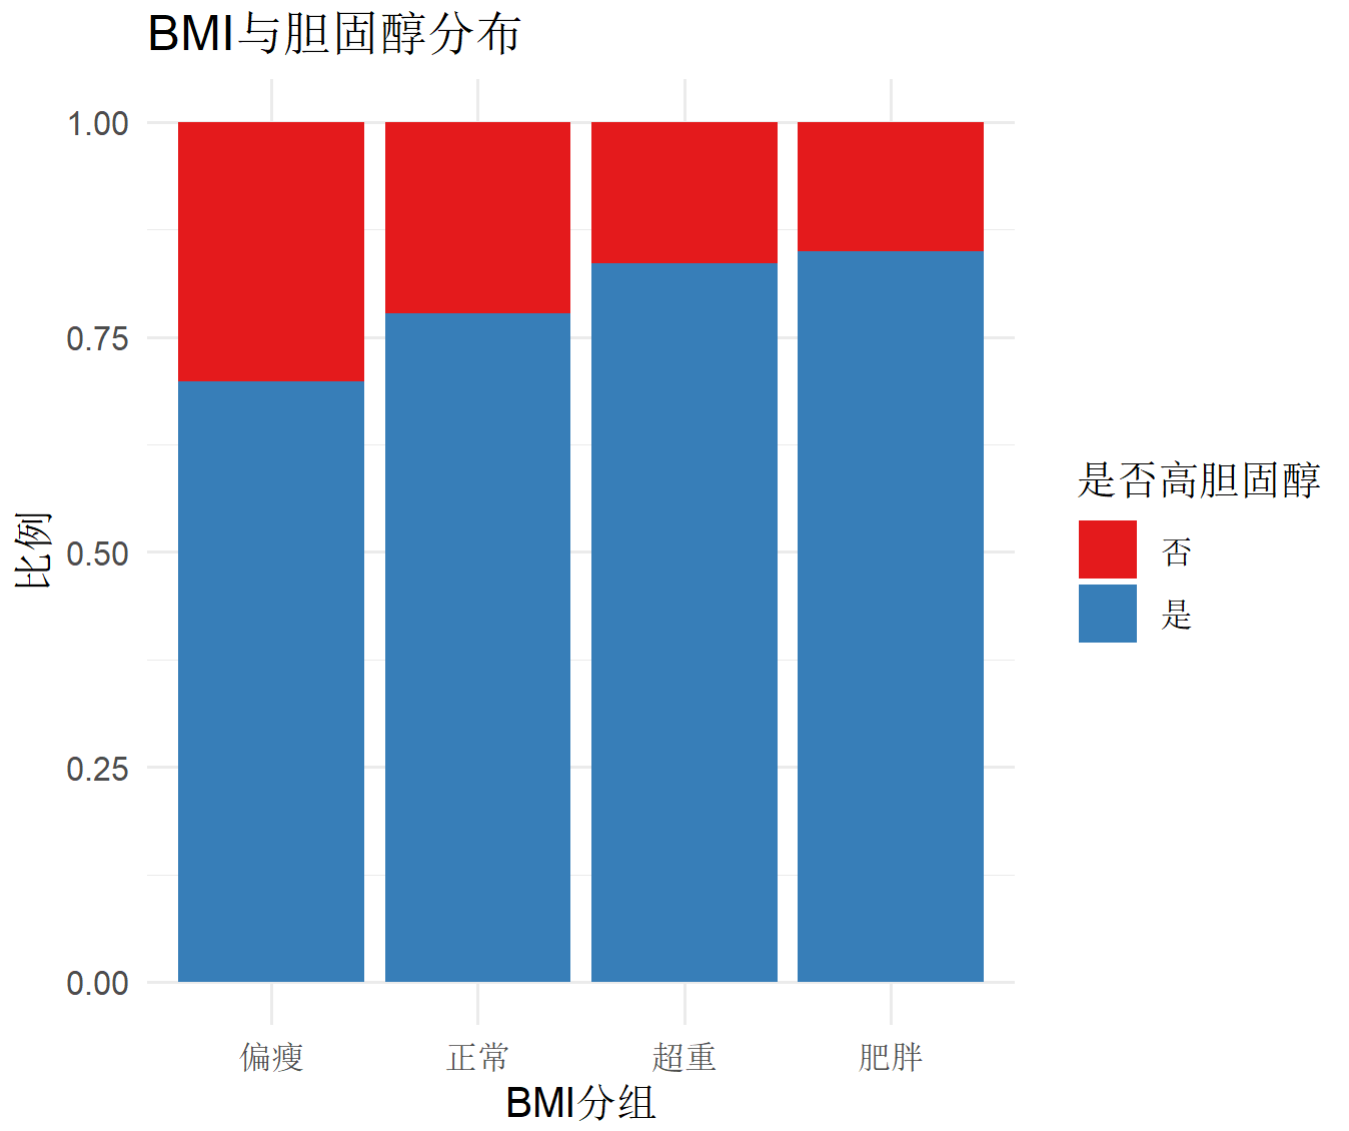
\includegraphics[width=0.7\textwidth]{figs/hw3_bmi_cholesterol_bar.png}
\end{center}

\begin{center}
\begin{tabular}{l|ccc}
 & 胆固醇 0 & 胆固醇 1 & Sum \\
\hline
偏瘦 & 48 & 111 & 159 \\
正常 & 783 & 2735 & 3518 \\
超重 & 720 & 3670 & 4390 \\
肥胖 & 399 & 2260 & 2659 \\
\hline
Sum & 1950 & 8776 & 10726 \\
\end{tabular}
\end{center}

使用 Pearson's Chi-squared test, $p\text{-value} < 2.2 \times 10^{-16}$

\subsubsection*{2. Age group}

\begin{center}
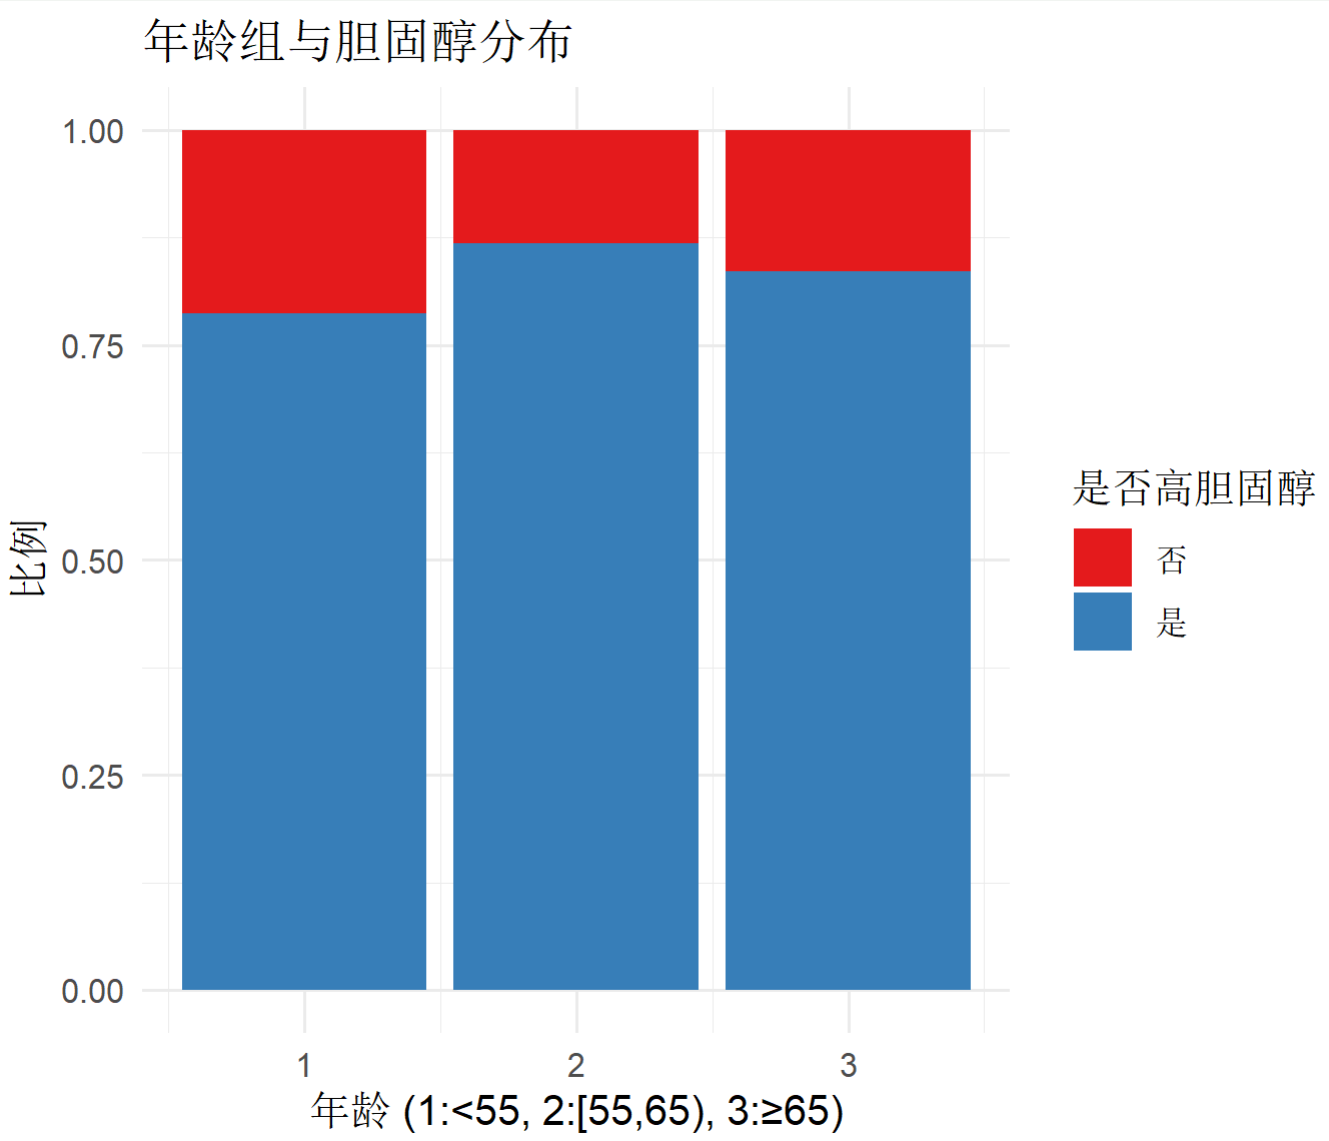
\includegraphics[width=0.7\textwidth]{figs/hw3_age_cholesterol_bar.png}
\end{center}

\begin{center}
\begin{tabular}{l|ccc}
 & totchol 0 & totchol 1 & Sum \\
\hline
1 ($<55$) & 1281 & 4716 & 5997 \\
2 ($[55,65)$) & 424 & 2809 & 3233 \\
3 ($\geq 65$) & 245 & 1251 & 1496 \\
\hline
Sum & 1950 & 8776 & 10726 \\
\end{tabular}
\end{center}

使用 Pearson's Chi-squared test, $p\text{-value} < 2.2 \times 10^{-16}$

\subsubsection*{3. Sex}

\begin{center}
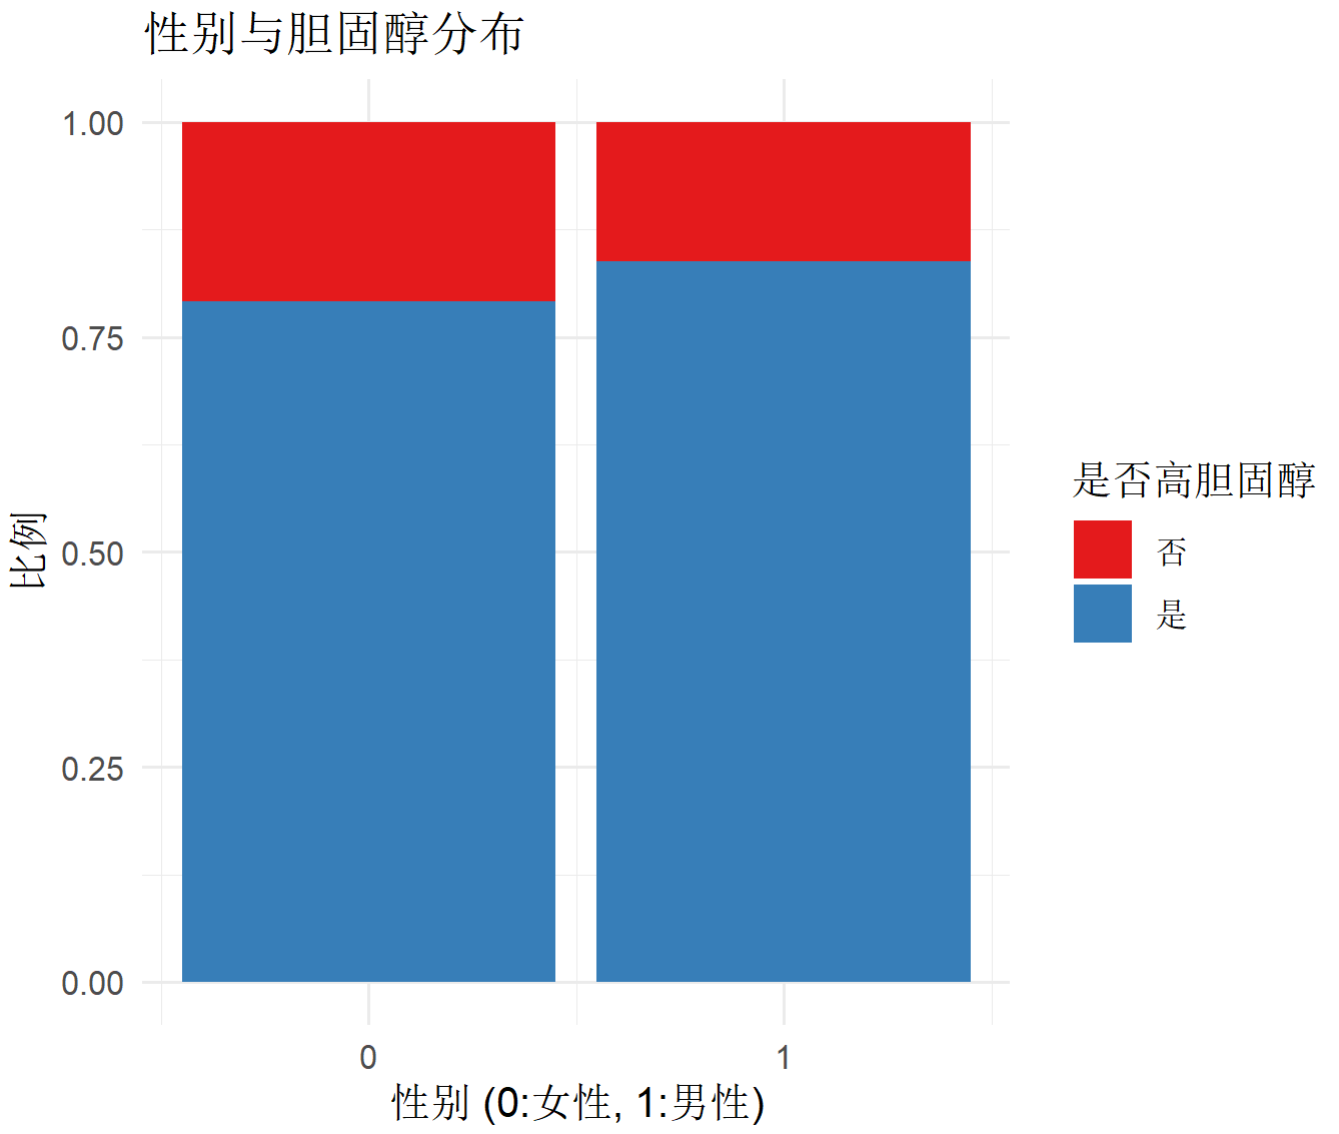
\includegraphics[width=0.7\textwidth]{figs/hw3_sex_cholesterol_bar.png}
\end{center}

\begin{center}
\begin{tabular}{l|ccc}
 & totchol 0 & totchol 1 & Sum \\
\hline
0 (female) & 967 & 3665 & 4632 \\
1 (male) & 983 & 5111 & 6094 \\
\hline
Sum & 1950 & 8776 & 10726 \\
\end{tabular}
\end{center}

使用 Pearson's Chi-squared test, $p\text{-value} = 3.23 \times 10^{-10}$

\subsubsection*{(c) Interpret}

以上三组均有 $p\text{-value} < 0.05$，拒绝零假设，即认为比较的两组变量有相关性。具体地，BMI 大的人比 BMI 小的人更可能有高胆固醇，老年人群比较年轻的人群更可能有高胆固醇，男性比女性更可能有高胆固醇。

此外，由于 BMI 的取值为连续变量，又在次前作业里检验过 BMI 的分布严重偏离正态，故我们可以选用 Wilcoxon rank sum test。

\begin{center}
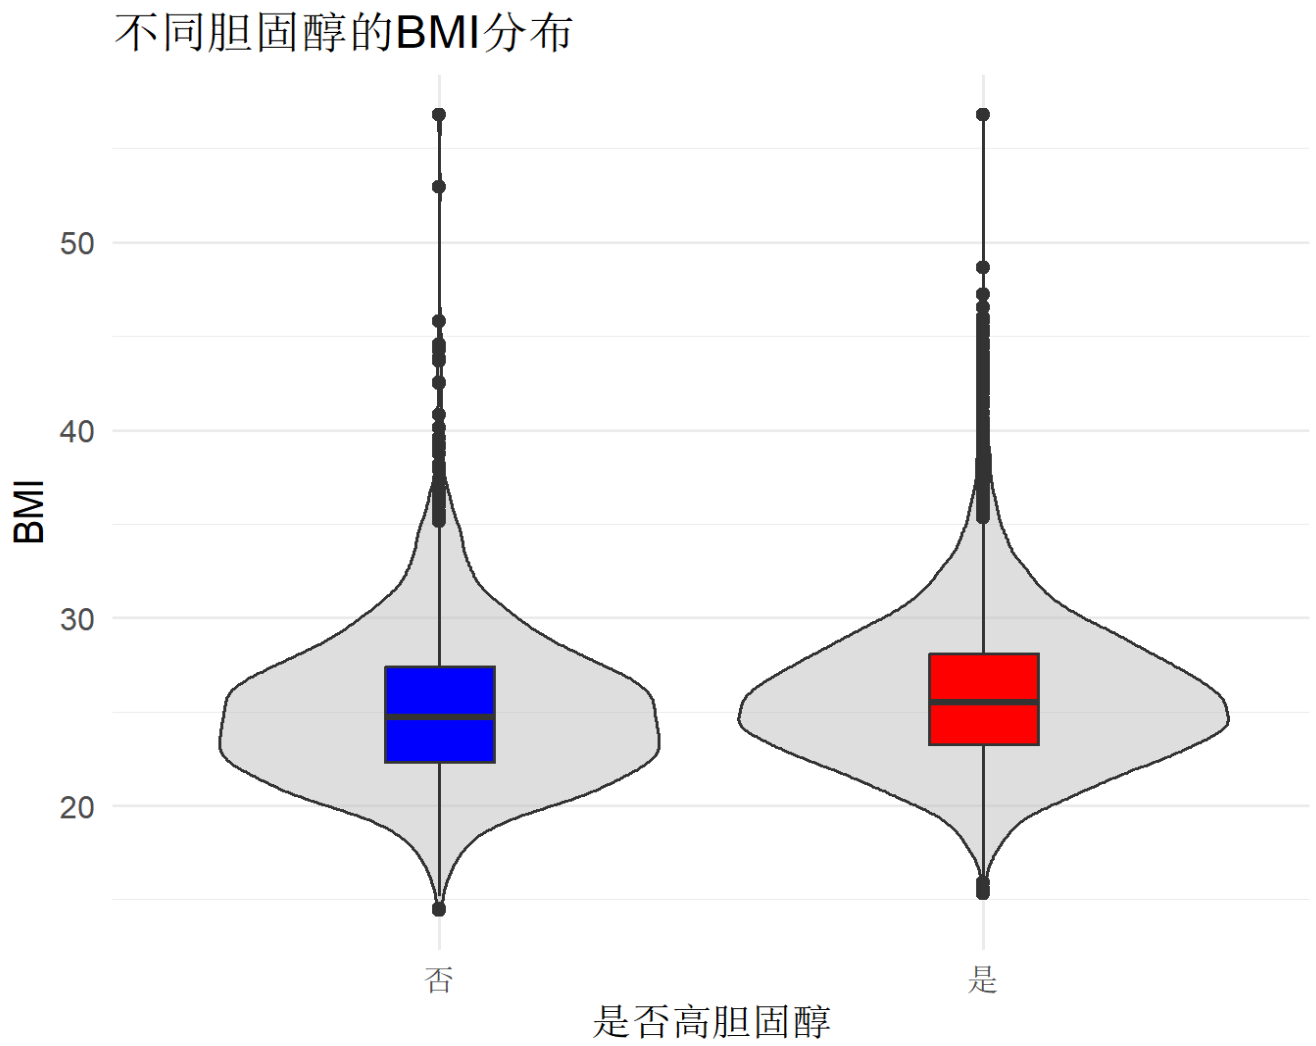
\includegraphics[width=0.7\textwidth]{figs/hw3_bmi_violin.png}
\end{center}

Wilcoxon rank sum test 结果：
\begin{verbatim}
p-value < 2.2e-16
alternative hypothesis: true location shift is not equal to 0
\end{verbatim}

\textbf{注：}

1. 对所用列的缺失数据采取了整行删除处理。

2. 前面部分如果否用蓝色是用红色可能更符合直觉，但因为还是不熟悉 ggplot，本次作业先不修改了。

3. 代码见下：

\begin{lstlisting}[language=R]
library(ggplot2)
df <- read.csv("Framingham_data.csv")
dfclean <- df[!is.na(df$TOTCHOL) & !is.na(df$BMI)
              & !is.na(df$AGE_group) & !is.na(df$SEX), ]
dfclean$bi_chole <- ifelse(dfclean$TOTCHOL > 200, 1, 0)

# a visualize (figures & tables)
# BMI (BMI也分组)
dfclean$bmigroup <- cut(
  dfclean$BMI,
  breaks = c(-Inf, 18.5, 24, 28, Inf),
  labels = c("偏瘦", "正常", "超重", "肥胖")
)
ggplot(dfclean, aes(x = bmigroup, fill = factor(bi_chole))) +
  geom_bar(position = "fill") +
  labs(title = "BMI与胆固醇分布",
       x = "BMI分组", y = "比例", fill = "是否高胆固醇") +
  scale_fill_brewer(labels = c("否", "是"), palette = "Set1") +
  theme_minimal()

b <- table("BMI" = dfclean$bmigroup,
           "胆固醇" = dfclean$bi_chole)
addmargins(b)
chisq.test(b)

# age
ggplot(dfclean, aes(x = AGE_group, fill = factor(bi_chole))) +
  geom_bar(position = "fill") +
  labs(title = "年龄组与胆固醇分布",
       x = "年龄 (1:<55, 2:[55,65), 3:≥65)",
       y = "比例", fill = "是否高胆固醇") +
  scale_fill_brewer(labels = c("否", "是"), palette = "Set1") +
  theme_minimal()

a <- table("age group" = dfclean$AGE_group,
           "totchol" = dfclean$bi_chole)
addmargins(a)
chisq.test(a)

# sex
ggplot(dfclean, aes(x = SEX, fill = factor(bi_chole))) +
  geom_bar(position = "fill") +
  labs(title = "性别与胆固醇分布",
       x = "性别 (0:女性, 1:男性)", y = "比例",
       fill = "是否高胆固醇") +
  scale_fill_brewer(labels = c("否", "是"), palette = "Set1") +
  scale_x_continuous(breaks = c(0, 1)) +
  theme_minimal()

s <- table("sex" = dfclean$SEX,
           "totchol" = dfclean$bi_chole)
addmargins(s)
chisq.test(s)

# 连续BMI
ggplot(dfclean, aes(x = factor(bi_chole, labels = c("否","是")),
                    y = BMI)) +
  geom_violin(fill = "gray", alpha = 0.5) +
  geom_boxplot(fill = c("blue", "red"), width = 0.2) +
  labs(title = "不同胆固醇的BMI分布",
       x = "是否高胆固醇", y = "BMI") +
  theme_minimal()
wilcox.test(dfclean$BMI ~ dfclean$bi_chole)
\end{lstlisting}
